%
% kegelschnitt.tex
%
% (c) 2021 Prof Dr Andreas Müller, OST Ostschweizer Fachhochschule
%
\documentclass[tikz]{standalone}
\usepackage{times}
\usepackage{amsmath}
\usepackage{txfonts}
\usepackage[utf8]{inputenc}
\usepackage{graphics}
\usetikzlibrary{arrows,intersections,math,calc}
\usepackage{ifthen}
\begin{document}

\definecolor{kegelfarbe}{rgb}{0.2,0.6,0.6}
\definecolor{ebenenfarbe}{rgb}{0.6,0.4,0.2}
\definecolor{fokusfarbe}{rgb}{0.8,0.0,0.0}
\definecolor{scheitelfarbe}{rgb}{0,0.6,0}
\definecolor{leitfarbe}{rgb}{0.8,0.2,0.8}
\definecolor{mantelfarbe}{rgb}{0.2,0.6,1.0}

\newboolean{showgrid}
\setboolean{showgrid}{false}
\def\breite{7}
\def\hoehe{5}

\begin{tikzpicture}[>=latex,thick]

% Povray Bild
\node at (0,0) {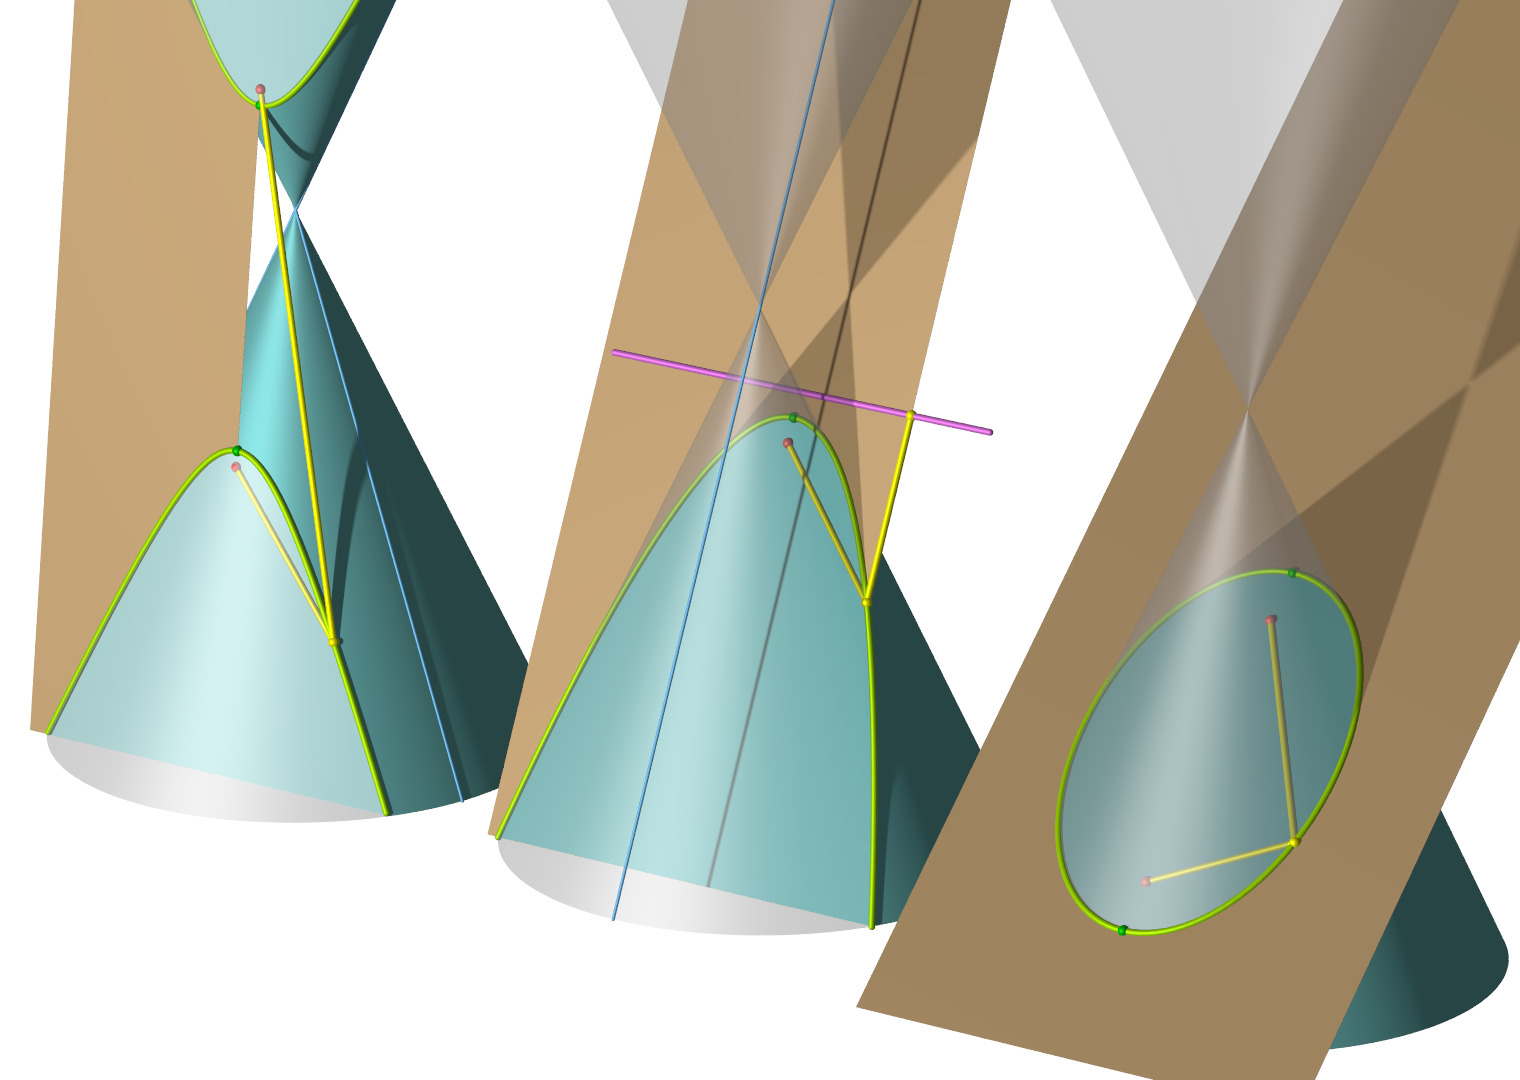
\includegraphics[width=14cm]{kegelschnitte.jpg}};

% Gitter
\ifthenelse{\boolean{showgrid}}{
\draw[step=0.1,line width=0.1pt] (-\breite,-\hoehe) grid (\breite, \hoehe);
\draw[step=0.5,line width=0.4pt] (-\breite,-\hoehe) grid (\breite, \hoehe);
\draw                            (-\breite,-\hoehe) grid (\breite, \hoehe);
\fill (0,0) circle[radius=0.05];
}{}

%
% Lage der Schnittebene
%
\begin{scope}[yshift=-7.5cm]
	% Hyperbel
	\begin{scope}[xshift=-4.5cm]
		\clip (-2,-2.5) rectangle (2,1.5);
		\fill[color=kegelfarbe!40]
			(-1.4,-3) -- (1.4,-3) -- (-1.4,3) -- (1.4,3) -- cycle;
		\begin{scope}[xshift=-0.3cm]
			\draw[color=ebenenfarbe,line width=1.4pt]
				(-0.4,-3) -- (0.4,3);
		\end{scope}
		\begin{scope}
			\draw[color=mantelfarbe,line width=1.2pt]
				(-0.4,-3) -- (0.4,3);
		\end{scope}
	\end{scope}

	% Parabel
	\begin{scope}
		\clip (-2,-2.5) rectangle (2,1.5);
		\fill[color=kegelfarbe!40]
			(-1.4,-3) -- (1.4,-3) -- (-1.4,3) -- (1.4,3) -- cycle;
		\begin{scope}[xshift=0.5cm]
			\draw[color=ebenenfarbe,line width=1.4pt]
				(-1.4,-3) -- (1.4,3);
		\end{scope}
		\begin{scope}
			\draw[color=mantelfarbe,line width=1.2pt]
				(-1.4,-3) -- (1.4,3);
		\end{scope}
	\end{scope}

	% Ellipse
	\begin{scope}[xshift=4.5cm]
		\clip (-2,-2.5) rectangle (2,1.5);
		\fill[color=kegelfarbe!40]
			(-1.4,-3) -- (1.4,-3) -- (-1.4,3) -- (1.4,3) -- cycle;
		\begin{scope}[xshift=0.9cm]
			\draw[color=ebenenfarbe,line width=1.4pt]
				(-3.4,-3) -- (3.4,3);
		\end{scope}
	\end{scope}

\end{scope}

%
% Beschriftung der 3D-Abbildung
%
\def\marke#1#2#3#4{
	\fill[color=white,opacity=0.5]
		({#1-0.25},{#2-0.2}) rectangle ({#1+0.20},{#2+0.2});
	\node[color=#3] at ({#1},{#2}) {#4};
}

\node[color=fokusfarbe] at (-5,0.5) {$F_1$};
\node[color=fokusfarbe] at (-4.5,4.4) {$F_2$};
%\node[color=scheitelfarbe] at (-4.5,4.1) [below left] {$S_2$};
%\node[color=scheitelfarbe] at (-4.7,0.8) [above left] {$S_1$};
\marke{-4.9}{3.7}{scheitelfarbe}{$S_2$}
\marke{-5.1}{1.1}{scheitelfarbe}{$S_1$}
\node[color=yellow] at (-3.9,-0.9) [right] {$P$};

\node[color=fokusfarbe] at (0.05,0.75) {$F$};
%\node[color=scheitelfarbe] at (0.4,1.0) [above left] {$S$};
\marke{0.35}{1.4}{scheitelfarbe}{$S$};
\node[color=yellow] at (0.95,-0.6) [right] {$P$};
\node[color=leitfarbe] at (2.2,1.2) {$l$};

\node[color=fokusfarbe] at (3.5,-2.9) {$F_1$};
\node[color=fokusfarbe] at (4.4,-0.8) {$F_2$};
%\node[color=scheitelfarbe] at (3.6,-3.5) [below left] {$S_1$};
%\node[color=scheitelfarbe] at (4.8,-0.4) [above right] {$S_2$};
\marke{3.05}{-3.85}{scheitelfarbe}{$S_1$}
\marke{5.3}{-0.0}{scheitelfarbe}{$S_2$}
\node[color=yellow] at (4.8,-2.7) [below right] {$P$};

%
% Beschriftung und geometrische Örter
%
\begin{scope}[yshift=-5.5cm]
	\node at (-4.5,0)
	{Hyperbel: $\overline{F_1P}-\overline{F_2P}=\text{const}$\strut};

	\fill[color=white,opacity=0.7] (-1.3,-0.25) rectangle (1.3,0.25);
	\node at (0,0) {Parabel: $\overline{FP}=\overline{lP}$\strut};

	\fill[color=white,opacity=0.7] (2.4,-0.25) rectangle (6.6,0.25);
	\node at (4.5,0)
	{Ellipse: $\overline{F_1P}+\overline{F_2P}=\text{const}$\strut};
\end{scope}

\end{tikzpicture}

\end{document}

